\documentclass[10pt,twocolumn,letterpaper]{article}

\usepackage{fgrebuttal}
\usepackage{times}
\usepackage{epsfig}
\usepackage{graphicx}
\usepackage{amsmath}
\usepackage{amssymb}
\usepackage{subfig}
\usepackage{subcaption}
\usepackage{pifont}% http://ctan.org/pkg/pifont
\usepackage{comment}
\usepackage{tabularx, booktabs, ragged2e}
\usepackage[acronym]{glossaries}
\usepackage{acronym}
\usepackage[pagebackref=true,breaklinks=true,letterpaper=true,colorlinks,bookmarks=false]{hyperref}

\def\cvprPaperID{41} 
\def\httilde{\mbox{\tt\raisebox{-.5ex}{\symbol{126}}}}

\newcommand{\xmark}{\ding{56}}%
\newcommand{\checkc}{\ding{51}}%
\newcommand{\NA}{---}
\newacronym{lfw}{LFW}{Labeled Faces in the Wild}
\newacronym{bfw}{BFW}{Balanced Faces In the Wild}
\newacronym{rfw}{RFW}{Racial Faces in-the-Wild:}
\newacronym{dp}{DemogPairs}{Demographic Pairs}

\newacronym{af}{AF}{\textit{Asian}-\textit{Female}}
\newacronym{am}{AM}{\textit{Asian}-\textit{Male}}
\newacronym{bf}{BF}{\textit{Black}-\textit{Female}}
\newacronym{bm}{BM}{\textit{Black}-\textit{Male}}
\newacronym{if}{IF}{\textit{Indian}-\textit{Female}}
\newacronym{im}{IM}{\textit{Indian}-\textit{Male}}
\newacronym{wf}{WF}{\textit{White}-\textit{Female}}
\newacronym{wm}{WM}{\textit{White}-\textit{Male}}
\newcommand{\com}[1]{\textcolor{red}{#1}}
\newcommand{\ie}{\textit{i}.\textit{e}., }
\newcommand{\eg}{\textit{e}.\textit{g}., }
\newcommand*{\etc}{etc.\@\xspace}

\providecommand{\cq}[1]{\textcolor{blue}{#1}}
\providecommand{\cqr}[1]{\sout{\textcolor{blue}{#1}}}

\begin{document}

\title{Face Recognition: Too Bias, or Not Too Bias?}

\maketitle

% \begin{figure*}[t!]
%     \centering
%         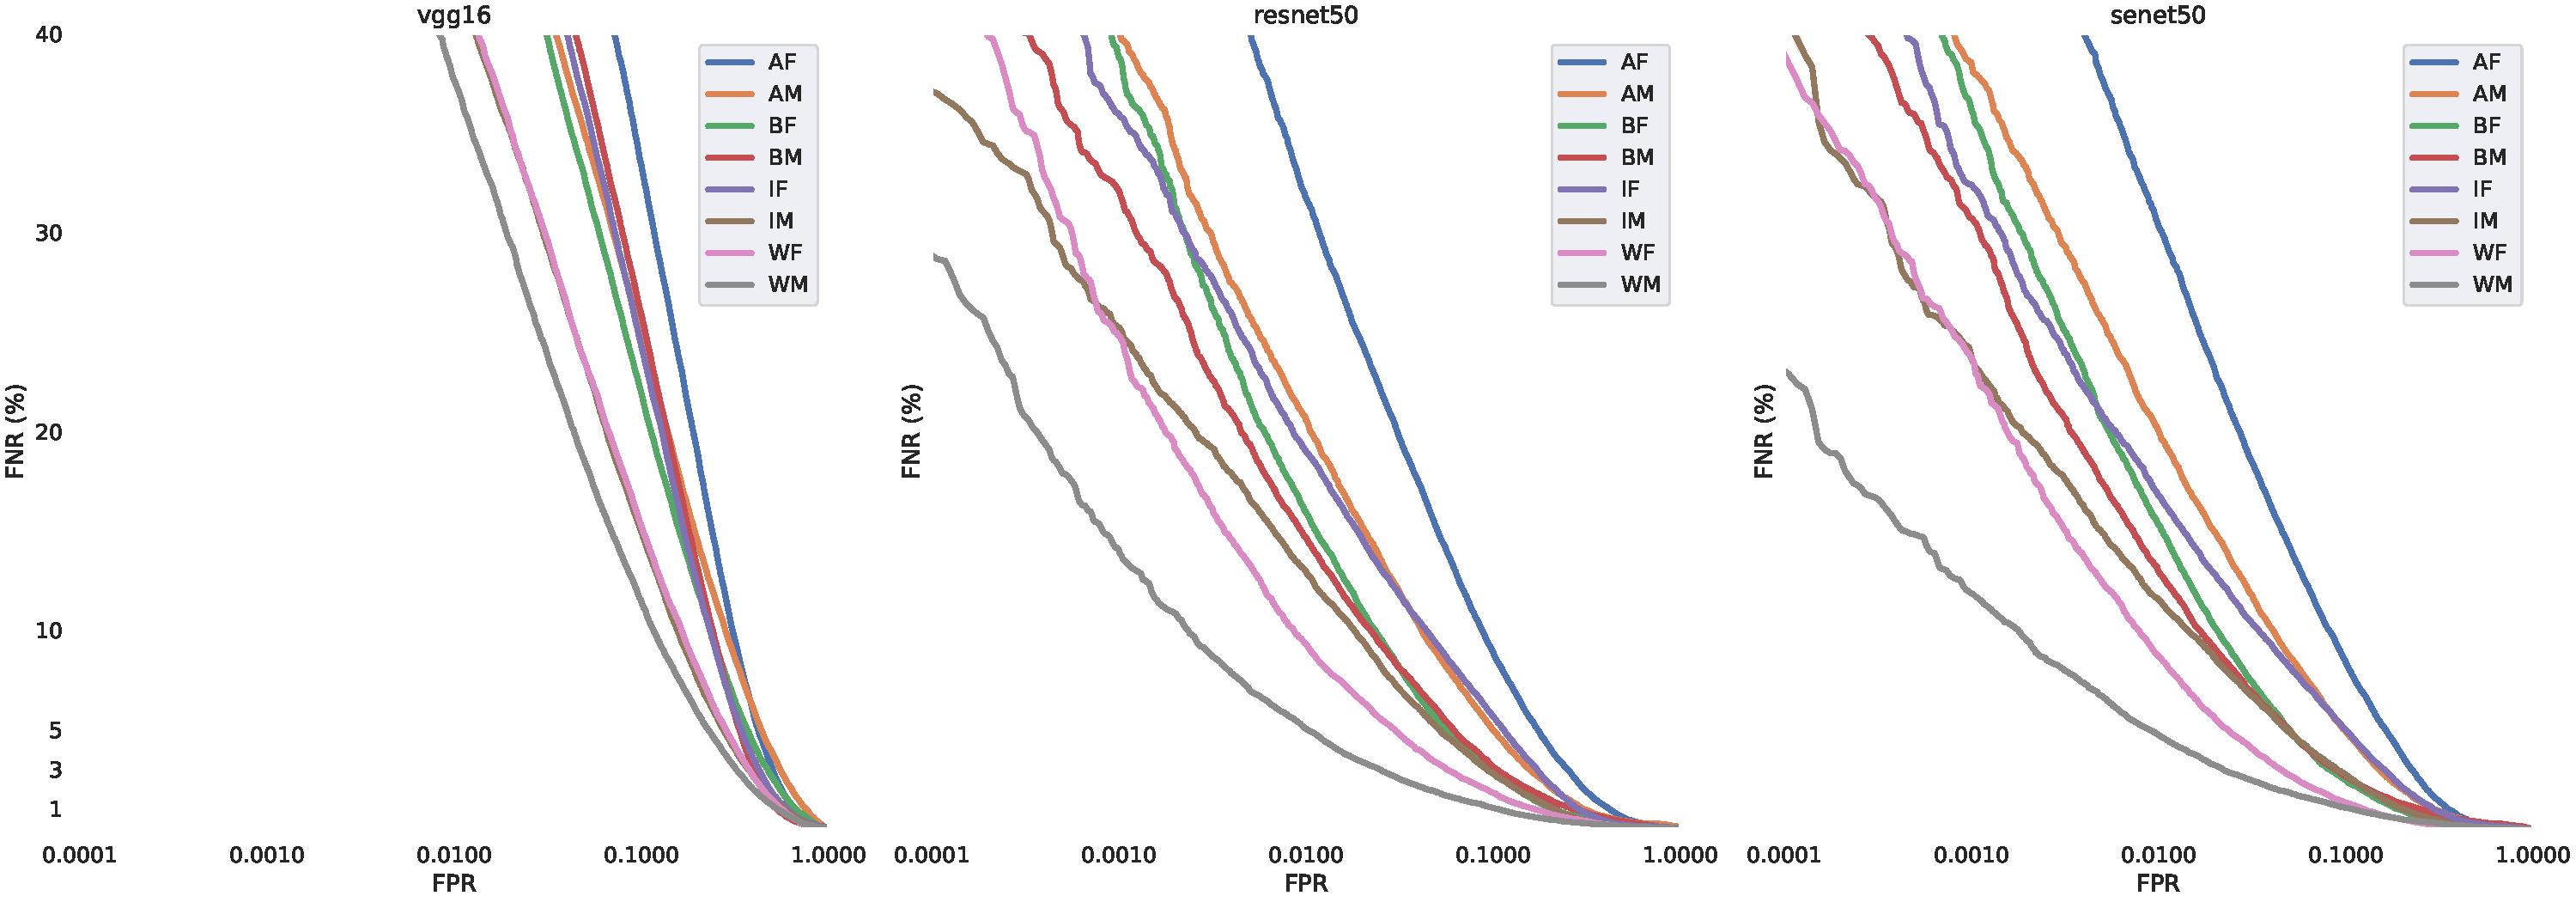
\includegraphics[width=.75\linewidth, trim={0mm 0mm 0mm 0mm},clip]{rebuttal/Figure1.pdf}
%     \caption{\textbf{DET curves for different CNN models}. FNR (vertical) vs FPR (horizontal) for different CNN-based models. The plots are displayed from lowest to best performance in terms of overall accuracy (\%) following the baseline (\ie global threshold). Notice that the better models have a larger variance in optimal thresholds from the global threshold.
%     }
    
%     \label{fig:fig1}
% \end{figure*}
\thispagestyle{empty}

\glsunset{bfw}
\glsunset{rfw}
\glsunset{dp}
% TODO DET curve: analyze threshold. Difference between models and global-- percent difference. Mention settings, simply how are they followed the same, but do state.

% \section{General Remarks}\label{sec:general}
% \noindent\textbf{Acknowledgement.} 
We thank reviewers for their time and comments. All reviewers agreed that bias in face recognition is important and well motivated in the paper. Two reviewers noted the value of the novel dataset to help find bias and improve performance. A reviewer noted the dataset will help motivate work in areas of bias, and another mentioned the urgency of finding a solution to bias and, thus, the importance of this work. Two reviewers noted that different optimal thresholds for subgroups is interesting, and the experiments showed it in results. A reviewer noted a thorough literature review. We begin by addressing four high-level issues noted by multiple reviewers, and then reply per reviewer:

\vspace{0.2mm}

\noindent\textbf{1. Additional CNN models} show bias results similar to ArcFace. As one example, (Fig.~\textcolor{red}{1}) shows DET curves (FNR vs FPR) for VggFace2 trained with 3 different backbones using (https://github.com/rcmalli/keras-vggface). Notice that the curves show similar trends across models, and consistent with  ArcFace (Fig. 2 in the paper). For example, the plots generated with ArcFace and VggFace2 all have the White Male curve at the bottom (best) and Asian Female on top (worst). In the paper, we initially chose to focus on ArcFace given the similarity of results to other networks. We will mention experiments with additional networks in paper, and refer readers to supplemental material for details.

\begin{table*}[t!]
\scriptsize
\glsreset{bfw}
\glsreset{rfw}
\glsreset{dp}
    \centering
    \begin{tabular}{rccccccc}%\toprule
    \multicolumn{2}{c}{Database} & \multicolumn{3}{c}{Number of}& \multicolumn{3}{c}{Balanced Labels}\\
    \cmidrule(lr){1-2}	\cmidrule(lr){3-5} \cmidrule(lr){6-8}
    Name & Source Data & Faces &  IDs & Subgroups & ID & Ethnicity & Gender\\\midrule
    \gls{dp}~\cite{demogPairs}     & CASIA-Web, VGG, VGG2 & 10,800& 600 & 6 &\checkc& \checkc &\checkc \\
    \gls{rfw}~\cite{wang2018racial}     &  MS-Celeb-1M &\approx80,000&\approx12,000& 4 & \xmark & \checkc &\xmark \\
    \gls{bfw} (ours) & VGG2 & 20,000 & 800 &8 & \checkc & \checkc &\checkc \\\bottomrule
    \end{tabular}
    \caption{\textbf{\gls{bfw} compared to related datasets.} \gls{bfw} is exactly balanced across ID, gender, and ethnicity: 25 faces of 100 subjects of 8 ethnic groups generate a list of 240,000 positive pairs (\ie  30,000 per subgroup). It is an extension of \gls{dp}, providing more samples per subject and more subgroups, and without the issues of missing data that occur when building \gls{dp}, with a majority of black females from CASIA-Web. For the reduction of potential conflict between train and test sets, \gls{bfw} was built solely with VGG2. \gls{rfw}, on the other hand, supports a different task (\ie domain adaptation). Furthermore, \gls{rfw} is made up of pairs labeled by subgroup and pair (\ie \{{\em match}, {\em non-match}\}), while not considering distribution of identities. }
    \label{tab:table1}
    % \vspace{-5mm}
\end{table*}


% \begin{table*}[t!]
% \scriptsize
% \glsreset{bfw}
% \glsreset{rfw}
% \glsreset{dp}
%     \centering
%     \begin{tabular}{rcccccccl}%\toprule
%     \multicolumn{2}{c}{Database} & \multicolumn{3}{c}{Number of}& \multicolumn{3}{c}{Balanced Labels}&\hspace{8mm} Task\\
%     \cmidrule(lr){1-2}	\cmidrule(lr){3-5} \cmidrule(lr){6-8}
%     Name & Source Data & Faces &  IDs & Subgroups & ID & Ethnicity & Gender\\\midrule
%     \gls{dp}~\cite{demogPairs}     & CASIA-Web, VGG, VGG2 & 10,800& 600 & 6 &\checkc& \checkc &\checkc& ID Verification \\
%     \gls{rfw}~\cite{wang2018racial}     &  MS-Celeb-1M &\approx80,000&\approx12,000& 4 & \xmark & \checkc &\xmark& Domain Adaptation \\
%     \gls{bfw} (ours) & VGG2 & 20,000 & 800 &8 & \checkc & \checkc &\checkc& ID Verification \\\bottomrule
%     \end{tabular}
%     \caption{\textbf{\gls{bfw} compared with related datasets.} \gls{bfw} is exactly balanced across ID, gender, and ethnicity. It is an extension of \gls{dp}, providing more samples per subject and the number of subgroups. Also, issues of missing data occur when building \gls{dp}, with a majority of black females from CASIA-Web. For this, the simplification, and the reduction of potential conflict between train and test sets, \gls{bfw} was built solely with VGG2. \gls{rfw}, on the other hand, supports a different task (\ie domain adaptation). Furthermore, \gls{rfw} is made up of pairs labeled by subgroup and pair (\ie \{{\em match}, {\em non-match}\}), while not including gender or considering the distribution of identities. In the end, \gls{bfw} is entirely balanced: 25 faces of 100 subjects of 8 ethnic groups are used to generate a list of 240,000 positive pairs (\ie  30,000 per subgroup).}
%     \label{tab:table1}
%     \vspace{-5mm}
% \end{table*}


\noindent\textbf{2. Data comparison} of the proposed \gls{bfw} with related datasets has been added to the paper (Table~\ref{tab:table1}). \gls{bfw} is designed such that each image includes identity, gender and ethnicity labels. Furthermore, there is an even number across all label-types. \gls{bfw}, unlike \gls{rfw}, splits ethnic-based subgroups by gender: subgroups based on ethnicity, on average, do vary with regards to optimal threshold. However, further splitting by gender yields gender-specific thresholds. Still, male faces are more separable than female counter-parts w.r.t subgroup, resulting in higher performances on average [line 620-622, col 1].

% (\ie \gls{dp}~\cite{demogPairs} and \gls{rfw}~\cite{wang2018racial}). 
\noindent\textbf{3. Details of human evaluation} regarding participants and survey were added to paper: To summarize, we recruited 120 subjects from multiple sources (\eg social media, email lists, and family/friends). Only white Americans ({\emph WA}) and Chinese from China ({\emph C}) were  targeted for this study. A total of 50 face pairs of non-famous subjects, with 20 ({\emph WA}) and 20 ({\emph C}) pairs (male and female split evenly). The other 10 pairs are of others (\eg Hispanic/ Latino, Japanese, African). Survey was created, distributed, and recorded via \href{https://paperform.co}{PaperForm}. The effort was supported by an IRB to ensure proper protocols were followed. A summary of results for every look-alike face pair is documented in the project repository, which will be made publicly available.

\noindent\textbf{4. Overarching Goal.} We created \gls{bfw} as a benchmark dataset for face verification of balanced data across subgroups. To aid this effort and ensure reproducibility, we created a Github repository, which includes easy-to-use notebook to regenerate all figures. We also have a project website with downloadable data, overview/ stats, and interactive gallery to browse \gls{bfw}. We are implementing \gls{bfw} as a Keras dataset for researchers. All will be released upon paper, publication: make entirely reproducible and maximize potential impact.

  
% The following sections are organized per reviewer. Please see the respective section for replies to individual remarks.

   
% \section{Review-Specific Rebuttal}
% \vspace{0.2mm}
\noindent\textbf{\textcolor{orange}{Reviewer1}}
\textbf{Q:} \textit{Analysis done with single CNN. The model bias can also be there to completely rely on the findings.Experiments using multiple CNNs would be great.} 
\textbf{A:} We have expanded the work with comparisons across multiple CNNs (Fig.~\textcolor{red}{1}). 
\textbf{Q:} \textit{How to improve performances of the FR system needs to be discussed.} 
\textbf{A:} We propose using variable thresholds based on the subgroup the individual belongs to. We compare the standard unique global threshold with the proposed variable threshold and demonstrate an improvement in performance [p6, Table II]. This shows significant improvement using our method (Table II). 
\textbf{Q:} \textit{We could do FR per subgroups as authors mention. Discussion or results from this for face verification (ROC) and face ID can be fruitful for research community.} 
\textbf{A:} We agree this is a promising research direction to build on work done here.



% \vspace{10mm}
\noindent\textbf{\textcolor{orange}{Reviewer2}}
\textbf{Q:} \textit{The presented threshold approach is evaluated in a very specific scenario. The extent of the evaluation is too narrow to derive general conclusions regarding bias in face verification neural networks. Only one network architecture is used to analyze the bias - ArcFace.} 
\textbf{A:} We have expanded the work with comparisons across multiple CNNs (Fig.~\textcolor{red}{1}). 
\textbf{Q:} \textit{ Only one similarity function is used to analyze the bias - cosine similarity.}  
\textbf{A:} We note that ArcFace produces L2-normalized embedding vectors for faces. As such, the cosine distance is proportional to the squared euclidean distance. Since distances are in the range [0, 1], the ranking of distances is preserved. As such, the metrics presented will not differ with euclidean distance, opposed to cosine distance. 
\textbf{Q:} \textit{Only one dataset is used to analyze the bias - BFW, introduced by the authors.} 
\textbf{A:} RFW provides balance in ethnicity labels and labels for pairs (\ie true or false). Thus, comparing results to another dataset is not possible, as we constructed this data by necessity (\ie RFW examines bias from the view of ethnicity classification, whereas we do identity verification).
Statistics and characteristics of the proposed \gls{bfw} to other face-based public datasets will be added to the paper to highlight the novelty in and need for data (Table~\ref{tab:table1}). 
\textbf{Q:} \textit{The different optimal thresholds for each subgroup is very interesting. However, the solution does not seem scalable to applications with growing, unbalanced datasets. Do we need to recompute when new identities are added to train set?} \textbf{A:} We note that if all subgroups are properly represented in the data when thresholds are computed, further data will not shift the overall distribution. We acknowledge that this method is difficult to employ when facing small datasets, as it may be difficult to compute the thresholds. However, this issue is encountered in many aspect of machine learning and isn't unique to our approach.
% \textbf{Q:} \textit{The human assessment experiment does not mention number of participants.} \textbf{A:} See (paragraph 3). 
\textbf{Q:} \textit{Face verification performance not compared to SOTA.} 
\textbf{A:} Our baseline is SOTA Arcface with a single global threshold, for which we show significant improvement over by using thresholds optimised per subgroup.
% facial verification with balance in ethnic backgrounds and gender-types. Thus, we propose this benchmark paper as a foundation for the research community.




\noindent\textbf{\textcolor{orange}{Reviewer3}}
\textbf{Q:} \textit{The paper is difficult to read and follow. There also exist several grammatical errors in the paper.} 
\textbf{A:} We have proofread and edited the paper to address this issue.
\textbf{Q:} \textit{they have proposed \gls{bfw} and that it is "complementary" to the existing \gls{rfw} dataset. It is not clear what additional contribution is being provided via the \gls{bfw} dataset, which extends the current literature. The authors must include a comparison with the \gls{rfw} dataset}
\textbf{A:} We have addressed this oversight by adding the requested comparison, see (Table~\ref{tab:table1}). We note that \gls{bfw} fundamentally differs from \gls{rfw} in its data and available types of label, although this was not made clear in our text. \gls{rfw} is intended as a benchmark in domain adaptation. Identity labels are not present, nor is a face verification benchmark. The task we address motivated us to build \gls{bfw}, a facial verification dataset with data balanced in terms of identity, gender, and ethnicity. \gls{bfw} supports the analysis and evaluation of 8 separate subgroups.
\textbf{Q:} \textit{There are no details with respect to training of Arcface when mentioned by authors.} 
\textbf{A:} We followed the same implementation as the authors of ArcFace, which achieves 99.83\% obtained on LFW. This will be clarified and detailed in paper.
% \textbf{Q:} \textit{In Section III.C, "Human performance was evaluated on face pairs focusing on two racial groups: Chinese and Caucasians." Where the data come from? Also, how many participants? How many pairs? How was study performed?}  \textbf{A:} See {\em General Remarks}, paragraph 3. 
\textbf{Q:} \textit{Fig. 4 presents the Rank-1 \% error. How is this calculated? Wasn't analysis drawn in terms of FAR and TAR?}  
\textbf{A:} FAR and TAR metrics are used to evaluate pairs of images. However, the Rank-1 analysis is not based on the pairs, but is the percent of faces for which the top-1 neighbor is of the same identity (effectively a top-1 accuracy). This analysis is performed within and across subgroups of gender and identity. We have explicitly stated and defined these metrics in the paper. 
\textbf{Q:} \textit{No clear description of how the category-based thresholds were obtained. A separate val set for obtaining thresholds?} 
\textbf{A:} We do a 5-fold cross validation protocol (Section IV.C, paragraph 2). Optimal thresholds were determined on train sets-- the threshold that resulted in lowest FPR w.r.t the desired FNR. All reported results are averaged across folds ($k=5$). Aforementioned will be updated and clearly stated.
    




{\footnotesize
\bibliographystyle{ieee}
\bibliography{rebuttal}
}
\end{document}
